% ============================================================
% LLM-BLM 実験 2：決算発表文のイベントの評価
% コンパイル：tectonic -X compile LLM-BLM_実験2.tex   （XeTeX 系。このフォルダで実行する）
% 図は 図/（作成スクリプト/figs.py が DB と experiments/E2_event_reaction/results から作る）
% 数値の出どころは experiments/E2_event_reaction/results/summary.json と findings.md、
% 事前登録は experiments/E2_event_reaction/preregistration.md、設計は リポジトリの 設計.md
% ============================================================
\documentclass[xelatex,ja=standard,jafont=haranoaji,a4paper,10pt,openany]{bxjsreport}
\setpagelayout*{left=24mm,right=24mm,top=24mm,bottom=26mm,footskip=11mm}

\usepackage{amsmath,amssymb,mathtools,bm}
\usepackage{booktabs,array,multirow,longtable}
\usepackage{graphicx}
\usepackage{adjustbox}
\usepackage{xcolor}
\usepackage{tikz}
\usetikzlibrary{arrows.meta,positioning,calc,fit}
\usepackage{enumitem}
\usepackage{caption}
\usepackage{float}
\usepackage[most]{tcolorbox}
\usepackage[hidelinks,bookmarksnumbered]{hyperref}
\pdfstringdefDisableCommands{\def\Omega{Ω}\def\tau{τ}\def\Sigma{Σ}}

\graphicspath{{図/}}

\definecolor{c1}{HTML}{2A78D6}
\definecolor{c2}{HTML}{EB6834}
\definecolor{c3}{HTML}{1BAF7A}
\definecolor{c4}{HTML}{EDA100}
\definecolor{c7}{HTML}{6250D6}
\definecolor{ink2}{HTML}{52514E}
\definecolor{soft1}{HTML}{E4EEF9}
\definecolor{soft2}{HTML}{FBEEDF}
\definecolor{soft3}{HTML}{E3F3E9}
\definecolor{soft4}{HTML}{EEE8FA}
\definecolor{soft5}{HTML}{FDF3DA}

\newcommand{\code}[1]{\texttt{#1}}
\newcommand{\SP}{S\&P500}
\newcommand{\figref}[1]{図~\ref{#1}}
\newcommand{\tabref}[1]{表~\ref{#1}}
\newcommand{\chapref}[1]{第~\ref{#1}~章}
\newcommand{\secref}[1]{\ref{#1}~節}

\setlist[itemize]{leftmargin=1.6em,itemsep=0.2em,topsep=0.4em}
\setlist[enumerate]{leftmargin=1.8em,itemsep=0.2em,topsep=0.4em}
\captionsetup{font=small,labelfont=bf,skip=6pt}
\renewcommand{\arraystretch}{1.2}
\setlength{\LTpre}{6pt}
\setlength{\LTpost}{6pt}

\makeatletter
\def\@makechapterhead#1{\vspace*{0.3\Cvs}{\parindent\z@\raggedright\normalfont
  \ifnum\c@secnumdepth>\m@ne\if@mainmatter{\Large\headfont\@chapapp\thechapter\@chappos}\par\nobreak\vskip0.4\Cvs\fi\fi
  \interlinepenalty\@M\LARGE\headfont #1\par\nobreak\vskip 1.5\Cvs}}
\def\@makeschapterhead#1{\vspace*{0.3\Cvs}{\parindent\z@\raggedright\normalfont
  \interlinepenalty\@M\LARGE\headfont #1\par\nobreak\vskip 1.5\Cvs}}
\makeatother

\newtcolorbox{keybox}[1][要点]{enhanced,breakable,colback=soft1,colframe=c1,boxrule=0.5pt,arc=2pt,
  left=8pt,right=8pt,top=6pt,bottom=6pt,title={#1},fonttitle=\sffamily\bfseries\small,coltitle=white}
\newtcolorbox{notebox}[1][注意]{enhanced,breakable,colback=soft2,colframe=c2,boxrule=0.5pt,arc=2pt,
  left=8pt,right=8pt,top=6pt,bottom=6pt,title={#1},fonttitle=\sffamily\bfseries\small,coltitle=white}
\newtcolorbox{verdict}[1][判定]{enhanced,breakable,colback=soft4,colframe=c7,boxrule=0.5pt,arc=2pt,
  left=8pt,right=8pt,top=6pt,bottom=6pt,title={#1},fonttitle=\sffamily\bfseries\small,coltitle=white}

\tikzset{
  box/.style={draw=#1,fill=#1!8,rounded corners=2pt,align=center,font=\footnotesize,inner sep=4pt,
              minimum height=10mm,text width=24mm},
  arr/.style={-{Stealth[length=2mm]},color=ink2,line width=0.6pt},
}

\title{LLM-BLM 実験 2\\[6pt]
  \large LLM が決算発表文から読み取る判断は、\\発表への株価の反応を説明するか：事前登録したイベントの評価}
\author{実験の結果の報告書}
\date{2026 年 10 月 18 日}

\begin{document}
\maketitle

% ============================================================
\chapter*{概要}
\addcontentsline{toc}{chapter}{概要}

前回の実験（『LLM-BLM 実験結果レポート』、H01〜H07）で、LLM に翌月のリターンを数値で予想させる構成は、入力の写しで価値がないと分かった。LLM を使う意味が残っていたのは、決算発表文から読み取った点数だけだった。今回は、その点数を「月次の断面」ではなく「決算発表 1 本ごとのイベント」として評価した。評価の手順と判定の基準は、株価の反応を計算する前に文書とコードで固定し（事前登録）、1 回だけ実行した。

\begin{keybox}[主な結論]
\begin{itemize}
\item \textbf{gpt-4o-mini の点数は、発表への株価の反応をはっきり説明する（支持）。}点数が 1 標準偏差高いと、発表をはさむ 2 取引日の超過リターンは $+1.20\%$ 高い（95\% 区間 $+0.95$〜$+1.45\%$、$t$ 9.4）。同じ発表日の中で点数を入れ替えた対照 1,000 回では、実際を超えたものは 0 回だった。標本は 2023 年 11 月〜2026 年 8 月の 5,374 本で、gpt-4o-mini はこの期間の株価を知らない。
\item \textbf{LLM を使わない方法の情報を、LLM の点数がほぼ含んでいる。}FinBERT、TF-IDF＋リッジ、数値の驚き（SUE）は、それぞれ単独では反応を説明する。しかし LLM の点数と同時に入れると、文章の 3 つの方法の効果はほぼ 0 になった。LLM の効果は、FinBERT や TF-IDF の約 3 倍である。
\item \textbf{ただし、取引には使えない。}反応は発表の 2 日のうちに出て、その後の 2〜21 日目のドリフトは有意でない（$+0.10\%$、$t$ 0.8）。点数を知ったときには、株価はすでに動いている。
\item \textbf{先読みのない小さなモデル（ChronoGPT、1.55B）は、質問に答えさせる使い方ではほとんど読み取れない。}同じ標本で $+0.04\%$（$t$ 0.4）、2016〜2023 年の 14,204 本で $+0.09\%$（Holm の補正の後 $p=0.089$）。
\item 関連の確認として、BLM の共分散のノイズ除去（Marcenko--Pastur）を比べた。制約のない最小分散では効くが、BLM の最適化（空売りなし、TE の上限）では今の Ledoit--Wolf のほうがわずかに良かった（付録 \ref{app:x01}）。
\end{itemize}
\end{keybox}

\textbf{意味}：LLM は、決算発表文から「市場がどう受け取るか」を、辞書や FinBERT より正確に読み取れる。これは LLM の読む力の確かな証拠だが、発表の後に取引する戦略や、月次の BLM のビューの価値にはならない。前回の H06（翌月のリターンは説明できない）と、今回の結果は矛盾しない。

\setcounter{tocdepth}{1}
{\small\tableofcontents}

% ============================================================
\chapter{前回の結果と、問いの立て直し}\label{ch:intro}

\section{前回の実験から分かっていたこと}

前回の 7 つの仮説の検証（2024 年 3 月〜2026 年 8 月の 30 か月）で、次のことが分かった。

\begin{itemize}
\item LLM の翌月のリターンの数値予想は、渡した月の値動きの写しだった（決定係数 0.81）。写しを除いた固有の IC は $-0.004$。
\item 回答のばらつきは、誤差の大きさとしては使えない。BLM は、当たり具合で較正した $\Omega$ と TE の上限で設計どおりに動くが、成績は予想を並べ替えたビューと区別できなかった。
\item 決算発表文（8-K の EX-99.1）を gpt-4o-mini に読ませた点数は、直近の値動きをなぞらず、業績の伸びに沿っていた。しかし翌月のリターンに対する月次の検定では、30 か月で有意にならなかった（H06）。
\end{itemize}

\section{方針と文献調査}

前回の結果を受けて、次に何をするかの方針を Claude・GPT・Gemini の 3 者に独立に書かせて比べ、さらに Gemini Deep Research を加えた 4 者で先行研究を調べた（\code{資料集/03\_方針と文献調査/}）。3 者と文献が一致したのは、次の点である。

\begin{enumerate}
\item LLM に数値のリターンを予想させる構成はやめる。LLM は直近の値を外挿しすぎ、楽観に寄る（Chen ほか 2024）。
\item LLM の役割は、決算発表文から決まった形の判断（ガイダンスの変更、見通し、語調）を取り出すことに絞る。
\item 評価の単位を、月次の断面から決算発表ごとのイベントに移す。件数が増え、検出力が上がる。
\item LLM を使わない文章の分析（辞書、FinBERT、TF-IDF）と比べる。
\item 知識の期限より前の文章は、社名を伏せても記憶から復元されるので、gpt-4o-mini では確認に使えない（Lopez-Lira・Tang・Zhu 2025）。代わりに、年ごとに学習を区切って公開されている ChronoGPT（He ほか 2025）で読む。
\end{enumerate}

文献からは、方針を変える発見もあった。決算発表文の内容は、翌朝の寄り付きで株価に完全に反映される（Wu ほか 2025）。そこで、主な目的変数を「発表の後のドリフト」ではなく「発表への反応」にし、ドリフトは副次の分析にした。

\section{今回の問い}

\begin{verdict}[主な問い]
LLM（gpt-4o-mini）が決算発表文から取り出した判断は、数値の驚き（SUE など）と、LLM を使わない文章の分析（辞書・FinBERT・TF-IDF）を超えて、発表への株価の反応を説明するか。
\end{verdict}

副次の問いは、(S1) 発表の後のドリフトも予測するか、(S2・S3) 先読みのない ChronoGPT でも同じことが言えるか、(S4) 語調・見通し・ガイダンスのどれが効くか、の 4 つである。

% ============================================================
\chapter{データ}\label{ch:data}

\section{決算発表文}

SEC EDGAR から、\SP{} の構成銘柄（期間中に一度でも入った銘柄）の 8-K のうち、Item 2.02（決算の発表）を含むものを取得した。本文には、添付の EX-99.1（プレスリリース）を選んだ。

\begin{table}[htbp]
\centering
\caption{取得した決算発表と、評価に使った標本。}
\label{tab:data}
\small
\begin{tabular}{p{4.6cm}rp{6.6cm}}
\toprule
& 件数 & 備考 \\
\midrule
取得した 8-K（2015-01〜2026-08） & 28,447 & 本文が取れたもの 28,108 \\
基本の標本 & 23,056 & 提出日に \SP{} の構成銘柄、本文が EX-99、同じ銘柄・同じ日の重複を除く \\
標本 A（主） & 5,374 & 2023-11〜2026-08、gpt-4o-mini の点数あり、519 社、527 の発表日 \\
標本 B（副） & 14,204 & 2016-01〜2023-10、ChronoGPT の点数あり、514 社 \\
株価が欠けて除いた発表 & A：0、B：1,373 & B は上場廃止などで株価が取れない銘柄 \\
\bottomrule
\end{tabular}
\end{table}

すべて新しい DB の表（\code{earnings\_releases}、\code{release\_scores} など）に入れた。前回の H06 の 6,209 本と 5,429 本の点数も、この表に移した（件数と費用 3.31 ドルが記録と一致することを確かめた）。

\section{発表の時刻と、反応の日}

EDGAR の受理時刻（UTC）をニューヨーク時間に直し、時間帯で反応の日（\code{event\_date}、終値が初めて発表を織り込む取引日）を決めた。寄り前と場中の受理はその日、16 時以後の受理は次の取引日である。

\begin{figure}[htbp]
\centering
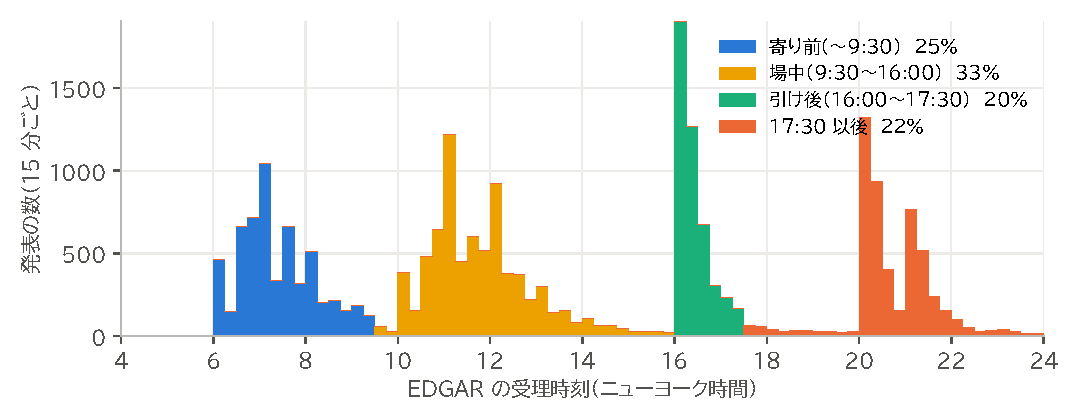
\includegraphics[width=0.95\linewidth]{timing.pdf}
\caption{EDGAR の受理時刻の分布（基本の標本 23,056 本）。山が 4 つあり、寄り前（6〜8 時）と場中（10〜13 時）、引け後（16 時台）と 17:30 以後（20〜21 時）が、それぞれ約 4 時間ずれて対になっている。}
\label{fig:timing}
\end{figure}

\figref{fig:timing} の 4 つの山は、多くの会社がプレスリリースを配信してから数時間後に 8-K を提出することを示している。「場中」の受理（33\%）の多くは寄り前に配信された発表で、その場合も反応の日は同じ日になる。「17:30 以後」（22\%）の多くは引け後に配信された発表で、反応の日は翌日になる。どちらも、主な窓（反応の日の前日の終値から、反応の日の翌日の終値まで）は配信の後の値動きを含む。場中の受理を除いても結果は変わらなかった（\chapref{ch:result}、R2）。

\section{数値の驚き}

アナリストの予想は持っていないので、数値の驚きは前年の同じ四半期との差で測った（季節のランダムウォーク）。

\begin{itemize}
\item \textbf{SUE}：希薄化後 EPS の前年同期との差を、過去 8 四半期の同じ差の標準偏差で割ったもの。過去は、発表の前に提出された四半期だけを使う。
\item \textbf{売上の驚き}：売上の前年同期比から、過去 4 四半期の前年同期比の平均を引いたもの。
\end{itemize}

SUE が計算できなかったのは標本 A の 5.2\%、売上の驚きは 3.3\% である。欠けは 0 で埋め、欠けを示す変数を回帰に入れた。

% ============================================================
\chapter{点数の付け方}\label{ch:scores}

同じ発表文に、5 つの方法で点数を付けた。結果を見る前に作れるもの（1〜4）は、事前登録の前にすべて計算した。TF-IDF は株価の反応で学習するので、事前登録の後に作った。

\begin{table}[htbp]
\centering
\caption{点数の付け方。時間は合計（この PC の GPU、RTX 5050 Laptop 8GB）。}
\label{tab:scorers}
\small
\begin{tabular}{p{2.6cm}p{6.6cm}p{2.0cm}p{2.4cm}}
\toprule
方法 & 中身 & 対象 & 費用・時間 \\
\midrule
gpt-4o-mini & H06 と同じ質問のまま。ガイダンスの変更・見通し・語調（$-2$〜$+2$）と、リスクの種類。温度 0。合成点数は 語調 ＋ 見通し ＋ ガイダンス（記載なしは 0） & 2023-11 以降 & 3.31 ドル（1.5 時間） \\
ChronoGPT & 発表の前の年末までの文章だけで学習した版（1.55B）。ガイダンスと語調の選択肢の確率を、中身のない文章での確率で割って較正。先頭の 1,792 トークンだけ読む & 全期間 & 0 円（8.3 時間） \\
辞書 & Loughran--McDonald の語彙で、肯定語と否定語の差 $\div$ 和。発表の年より後に辞書に加わった語は使わない & 全期間 & 0 円（6 分） \\
FinBERT & 金融の文章で学習した BERT。先頭の 200 文の、肯定の確率 $-$ 否定の確率の平均 & 全期間 & 0 円（4.2 時間） \\
TF-IDF＋リッジ & 語彙 2 万語。四半期ごとに、その四半期の始まりより前に窓が閉じた発表の反応で学び直す & 全期間 & 0 円（14 分） \\
\bottomrule
\end{tabular}
\end{table}

gpt-4o-mini の点数は楽観に寄る。語調は 88\% が前向き（$+1$ が 71\%、$+2$ が 17\%）、ガイダンスは 42\% が引き上げ、10\% が引き下げだった。発表文そのものが前向きに書かれるためで、回帰では標準化するので影響しない。点数どうしの順位相関は、LLM と FinBERT が 0.38、LLM と TF-IDF が 0.38、LLM と SUE が 0.28、LLM と ChronoGPT が 0.17 だった。

% ============================================================
\chapter{評価の方法と事前登録}\label{ch:method}

\section{事前登録}

前回の実験で探索した期間を再び使うので、結果を見てから手順を選ぶ余地をなくす必要がある。そこで、株価の反応を一度も計算しないうちに、次のものを 1 つのコミット（\code{2df746e}）に固定して GitHub にプッシュし、その後に 1 回だけ実行した。

\begin{itemize}
\item 事前登録の文書（\code{experiments/E2\_event\_reaction/preregistration.md}）：標本、変数、検定、判定の基準、副次の分析、頑健性の確認、実装の細部
\item 評価のコード（\code{run.py}）：作ったデータでだけテストしたもの
\item 使う点数の番号と、その設定のハッシュ
\end{itemize}

\section{主な検定}

\begin{itemize}
\item \textbf{目的変数}：反応の日の前日の終値から、翌日の終値まで（2 取引日）の超過リターン。超過リターンは、銘柄の配当込みのリターン $-$ 同じセクターの ETF のリターン。上下 1\% で丸める。
\item \textbf{主な説明変数}：gpt-4o-mini の合成点数（標準化）。
\item \textbf{統制}：SUE、売上の驚き（丸め、欠けの印つき）、辞書・FinBERT・TF-IDF の点数（標準化）、発表前 21 日の超過リターン、時価総額の対数。セクターと年・四半期の固定効果。
\item \textbf{標準誤差}：反応の日ごとにまとめる（同じ日の発表どうしの相関のため）。
\item \textbf{置換の対照}：同じ反応の日の中で点数を入れ替え、1,000 回回帰し直す。
\item \textbf{判定}：点数の係数が、t 検定と置換の両方で片側 $p<0.05$ なら「支持」。
\end{itemize}

副次の分析（S1〜S4、6 つの回帰）は Holm で補正した。頑健性の確認（R1〜R7）は判定に使わない。

% ============================================================
\chapter{結果}\label{ch:result}

\section{主な検定}

\begin{verdict}
\textbf{支持。}gpt-4o-mini の合成点数の係数は、1 標準偏差あたり $+120$bp（95\% 区間 $+95$〜$+145$bp、$t=9.41$、片側 $p=8\times10^{-20}$）。置換の対照の片側 $p=0.001$（1,000 回で実際を超えたのは 0 回で、出せる最小の値）。決定係数は、統制だけのモデルより 2.2 ポイント高い。
\end{verdict}

\begin{figure}[htbp]
\centering
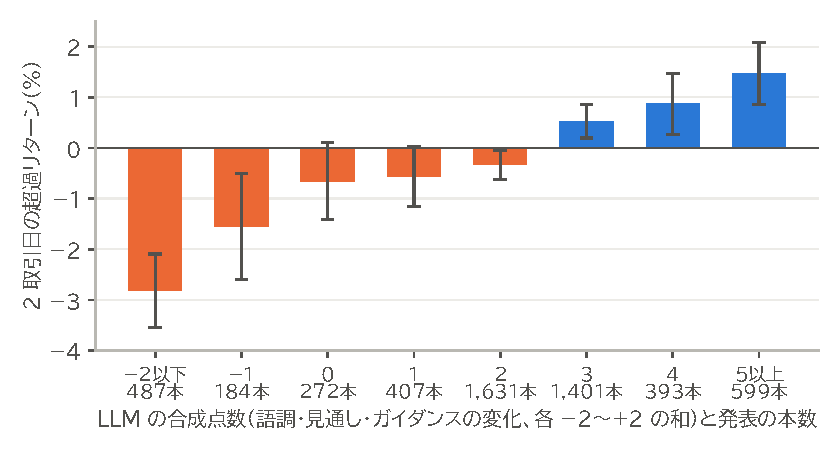
\includegraphics[width=0.66\linewidth]{quintile.pdf}
\caption{LLM の合成点数の値ごとの、2 取引日の超過リターンの平均（標本 A、上下 1\% で丸め、縦線は発表日でクラスタした 95\% 区間）。本数の少ない両端（$-5$〜$-2$、$5$〜$6$）はまとめた。探索の図で、判定には使っていない。}
\label{fig:quintile}
\end{figure}

合成点数の値ごとに並べると、反応の平均は $-2$ 以下で $-2.82\%$、$-1$ で $-1.55\%$、$0$ で $-0.65\%$、$1$ で $-0.57\%$、$2$ で $-0.33\%$、$3$ で $+0.53\%$、$4$ で $+0.87\%$、$5$ 以上で $+1.48\%$ と、点数の順に並んだ（\figref{fig:quintile}）。両端の差は約 4.3 ポイントである。

\begin{notebox}[図の作り直し（2026-10-28）]
この図は初め、点数の 5 分位（同じ点数の発表を、ファイルの中の順で機械的に割り振ったもの）で描いていた（平均は $-1.77\%$、$-0.20\%$、$-0.25\%$、$+0.46\%$、$+1.16\%$）。
合成点数は整数で、2 が 1,631 本、3 が 1,401 本と同じ値が多いので、2 番目と 3 番目の 5 分位はほぼ同じ「点数 2」の発表を分け合い、真ん中が平らに見えていた。
点数の値ごとの図に替えた。判定（回帰の係数）は変わらない。
\end{notebox}

\section{LLM を使わない方法との比較}

\begin{figure}[htbp]
\centering
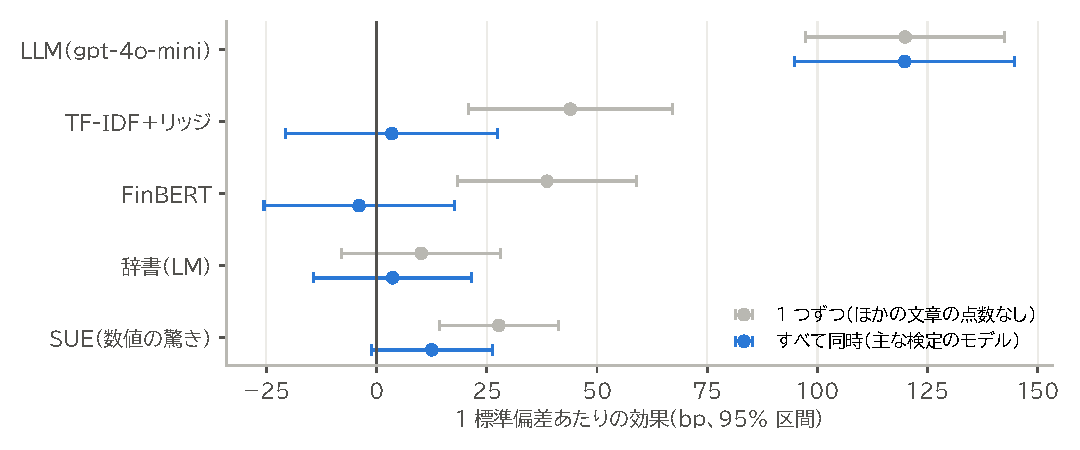
\includegraphics[width=0.95\linewidth]{compare.pdf}
\caption{点数ごとの効果（1 標準偏差あたり、95\% 区間）。灰色はほかの文章の点数を入れずに 1 つずつ（数値の驚きなどの統制は入れる）、青は主な検定のモデル（すべて同時）。探索の図。}
\label{fig:compare}
\end{figure}

1 つずつ入れると、TF-IDF（$+44$bp、$t$ 3.7）、FinBERT（$+39$bp、$t$ 3.7）、SUE（$+28$bp、$t$ 4.0）も反応を説明する。辞書は弱い（$+10$bp、$t$ 1.1）。しかし LLM の点数と同時に入れると、文章の 3 つの方法の係数は 0 に近くなる（$t$ 0.3、$-0.4$、0.4）。一方、LLM の係数は 1 つずつでも同時でも $+120$bp で変わらない（\figref{fig:compare}）。\textbf{LLM の点数は、ほかの文章の方法が持つ情報をほぼ含み、さらにその約 3 倍の情報を持つ。}Siano（2025）の「LLM による決算発表文の測度は、辞書や LLM でない機械学習の 3 倍、発表の短い期間のリターンを説明する」と合う。

\section{反応の後：ドリフト}

\begin{figure}[htbp]
\centering
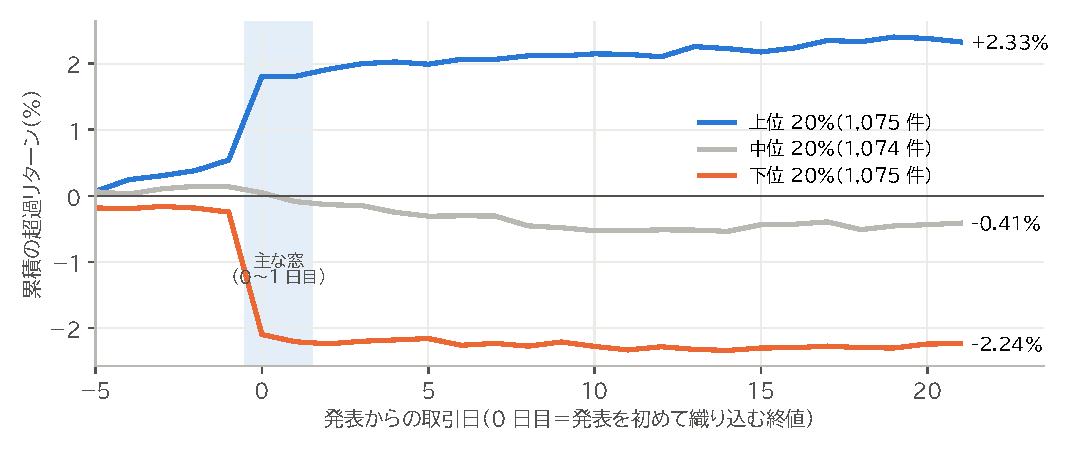
\includegraphics[width=0.95\linewidth]{car.pdf}
\caption{LLM の合成点数の上位・中位・下位 20\% の、累積の超過リターン（標本 A、丸めなし）。探索の図。}
\label{fig:car}
\end{figure}

反応の大部分は 0 日目に出る（\figref{fig:car}）。上位 20\% は 0〜1 日目で約 $+1.3\%$、下位 20\% は約 $-2.0\%$ 動き、その後はほぼ横ばいだった。上位は 21 日目までにさらに $+0.5\%$ ほど上がるが、統制を入れた回帰では、2〜21 日目のドリフトは有意でない（S1、$+10$bp、$t$ 0.83、Holm の $p=0.41$）。上位は発表の前（$-5$〜$-1$ 日目）にも約 $+0.5\%$ 上がっている。8-K の提出が配信より 1 日以上遅れた発表では、反応が $-1$ 日目に入るためと考えられる。窓を $[-1,+1]$ に広げても係数は同じ（$+120$bp）だった（R1）。

\section{副次の分析と頑健性}

\begin{figure}[htbp]
\centering
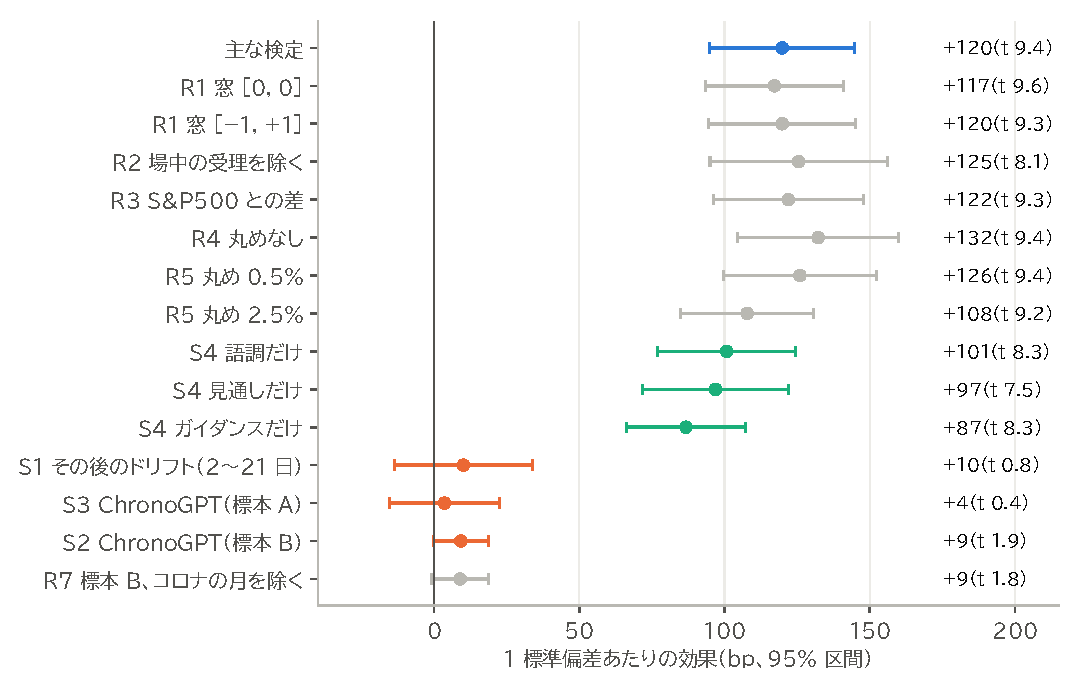
\includegraphics[width=0.95\linewidth]{forest.pdf}
\caption{主な検定（青）、頑健性の確認（灰）、語調・見通し・ガイダンスの 1 つずつ（緑）、ドリフトと ChronoGPT（橙）の係数と 95\% 区間。R6（順位の版）は単位が違うので省いた（$t$ 7.5）。}
\label{fig:forest}
\end{figure}

\begin{table}[htbp]
\centering
\caption{副次の分析（Holm で 6 つを補正）。係数は 1 標準偏差あたりの bp。}
\label{tab:secondary}
\small
\begin{tabular}{lrrrr}
\toprule
& 係数 & $t$ & Holm の $p$ & 件数 \\
\midrule
S1 発表の後のドリフト（2〜21 日目） & $+10$ & 0.83 & 0.41 & 5,374 \\
S2 標本 B（2016〜2023）を ChronoGPT で & $+9$ & 1.89 & 0.089 & 14,204 \\
S3 標本 A を ChronoGPT で & $+4$ & 0.37 & 0.41 & 5,374 \\
S4 語調だけ & $+101$ & 8.29 & $3\times10^{-15}$ & 5,374 \\
S4 見通しだけ & $+97$ & 7.55 & $4\times10^{-13}$ & 5,374 \\
S4 ガイダンスだけ & $+87$ & 8.26 & $3\times10^{-15}$ & 5,374 \\
\bottomrule
\end{tabular}
\end{table}

\begin{itemize}
\item \textbf{語調・見通し・ガイダンスは、どれも単独で強く効く}（S4）。合成点数の効果は、3 つのどれか 1 つから来ているのではない。
\item \textbf{頑健性}：窓を変えても（R1）、場中の受理を除いても（R2）、S\&P500 との差にしても（R3）、丸めをなくしても・幅を変えても（R4・R5）、順位に直しても（R6）、$t$ は 7.5〜9.6 の範囲に収まり、係数（単位の違う R6 を除く）は $+108$〜$+132$bp だった（\figref{fig:forest}）。結論は丸め方や窓の取り方に左右されない。
\item \textbf{ChronoGPT}：標本 B で $+9$bp（補正の前の片側 $p=0.03$、補正の後 0.089）、コロナの月を除いても $+9$bp（R7）。同じ標本 A では $+4$bp で、gpt-4o-mini の $+120$bp と大きな差がある。
\end{itemize}

% ============================================================
\chapter{考察}\label{ch:discussion}

\section{LLM は何を読み取っているか}

gpt-4o-mini の点数は、FinBERT や TF-IDF の情報をほぼ含み、その約 3 倍の情報を持っていた。FinBERT は文ごとの語調の平均、TF-IDF は単語の出方しか見ない。LLM は文書全体から「ガイダンスを引き上げたか」「需要は強まっているか」といった判断を読める。この差が、反応の説明力の差に表れたと考えられる。

一方で、数値の驚きの統制は弱い。アナリストの予想がないので、SUE は前年同期との差でしか測れていない。発表文には「予想を上回った」「市場の予想を下回るガイダンス」といった記述があり、LLM はこれを読んで本当の驚きを捉えている可能性がある。その場合、効果の一部は「文章から数値の驚きを読む力」で、純粋な語調の情報ではない。どちらでも LLM の読む力の証拠であることは変わらないが、「数値を超える情報」と言い切るには、ガイダンスの数値などで統制を強める必要がある。

\section{取引と BLM にとっての意味}

反応は発表の 2 日のうちにほぼ出尽くした。この点数が手に入るのは発表文を読んだ後なので、それから売買しても、反応の大部分はすでに株価に入っている。前回の H06 で翌月のリターンを説明できなかったことと、今回の結果は矛盾しない。どちらも「発表の内容は速やかに株価に織り込まれる」ことを示している（Wu ほか 2025、Yu ほか 2026）。

BLM のビューは「これから先のリターンの見込み」なので、この点数をそのままビューにしても価値は生まれない。BLM に組み込むかどうかは、ドリフトの部分（S1）が十分に大きいと示されてからにすべきである。

\section{先読みのないモデル}

ChronoGPT は、先読みがないことを学習データの段階で保証できる唯一の比べる相手だが、質問に答えさせる使い方（選択肢の確率）では、ほとんど読み取れなかった。1.55B と小さく、先頭の 1,792 トークンしか読めず、指示の学習のデータも 2000 年より前の内容に限られている。He ほか（2025）は、このモデルの内部の数値（最後の層）を取り出し、その上に過去のデータで学習した回帰を置く使い方で、大きなモデルと同程度の成績を報告している。標本 B（2016〜2023）で「LLM の読む力」を確かめるには、この方法でやり直す必要がある。

% ============================================================
\chapter{限界}\label{ch:limits}

\begin{itemize}
\item \textbf{数値の驚きの統制が弱い。}アナリストの予想がなく、SUE は前年同期との差で測った。
\item \textbf{主な標本は約 3 年。}gpt-4o-mini の知識の期限より後に限ったため（527 の発表日）。
\item \textbf{発表の時刻}：EDGAR の受理時刻を使い、プレスリリースの配信時刻は持っていない。8-K の提出が配信より 1 日以上遅れた発表では、反応の一部が窓の外に出る。場中の受理を除いても、窓を広げても結果は変わらなかった。
\item \textbf{生存者の偏り}：上場廃止などで株価が取れない銘柄は除いている（標本 B で 1,373 本）。
\item \textbf{ChronoGPT の弱さ}が、モデルの弱さか、質問の形の弱さかは区別できない。
\item \textbf{同じ期間の再利用}：標本 A は、前回の H06 で翌月のリターンについて一度見た期間である。発表への反応は一度も計算していなかったので、事前登録で手順を固定した。
\end{itemize}

% ============================================================
\chapter{次に行うこと}\label{ch:next}

リポジトリの \code{やること.md} に一覧がある。効果が大きいと考える順に挙げる。

\begin{enumerate}
\item \textbf{ChronoGPT の内部の数値と回帰}（He ほか 2025 の方法）。標本 B で、先読みのない比べる相手を強い形で作り直す。GPU で数時間（借りれば 1 時間程度）。
\item \textbf{数値の驚きの統制を強める}。発表文のガイダンスの数値（売上・EPS の見通し）と前回の見通しの差を、数値の驚きとして加える。「LLM は数値以外も読んでいるか」を確かめる。
\item \textbf{配信の時刻の確認}。受理と配信のずれを数十本で照合し、窓の決め方を確かめる。
\item \textbf{超過リターンの基準を良くする}。Fama--French の日次の因子で、市場・規模・バリュー・モメンタムを除く。
\item \textbf{BLM への組み込みは保留}。ドリフトが十分に大きいと示されるまで行わない。
\end{enumerate}

% ============================================================
\appendix
\chapter{共分散のノイズ除去（X01）}\label{app:x01}

待ち時間に、BLM の共分散 $\Sigma$ の推定を比べた（\code{experiments/X01\_covariance\_denoise/}）。LLM は使わない。2016〜2026 年の 127 か月の月末に、約 460 銘柄で比率を決め、翌月の値動きで答え合わせした。比べ方は計算の前に固定した。

\begin{figure}[H]
\centering
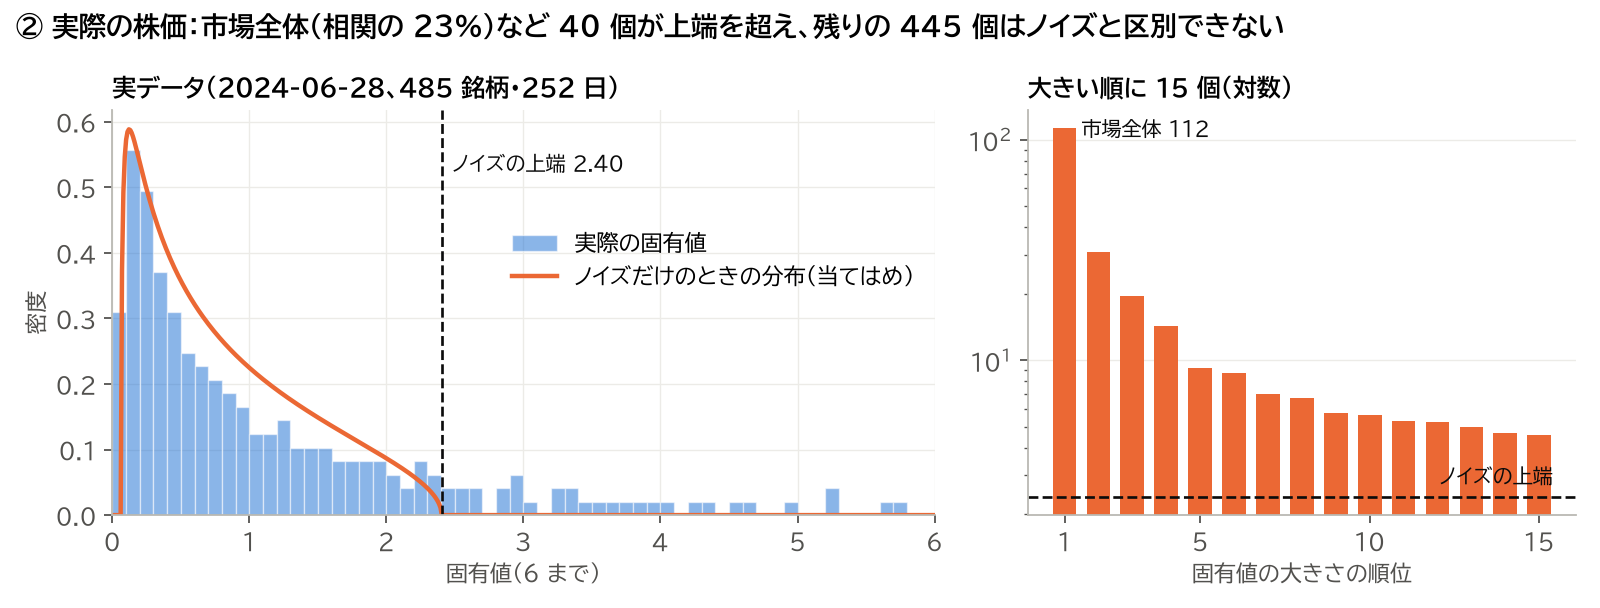
\includegraphics[width=0.98\linewidth]{x01_2_real_eigenvalues.png}
\caption{2024 年 6 月末の \SP{} の相関行列の固有値。Marcenko--Pastur のノイズの上端（2.40）を超えるのは 40 個で、残りの 445 個はノイズと区別できない。}
\end{figure}

\begin{figure}[H]
\centering
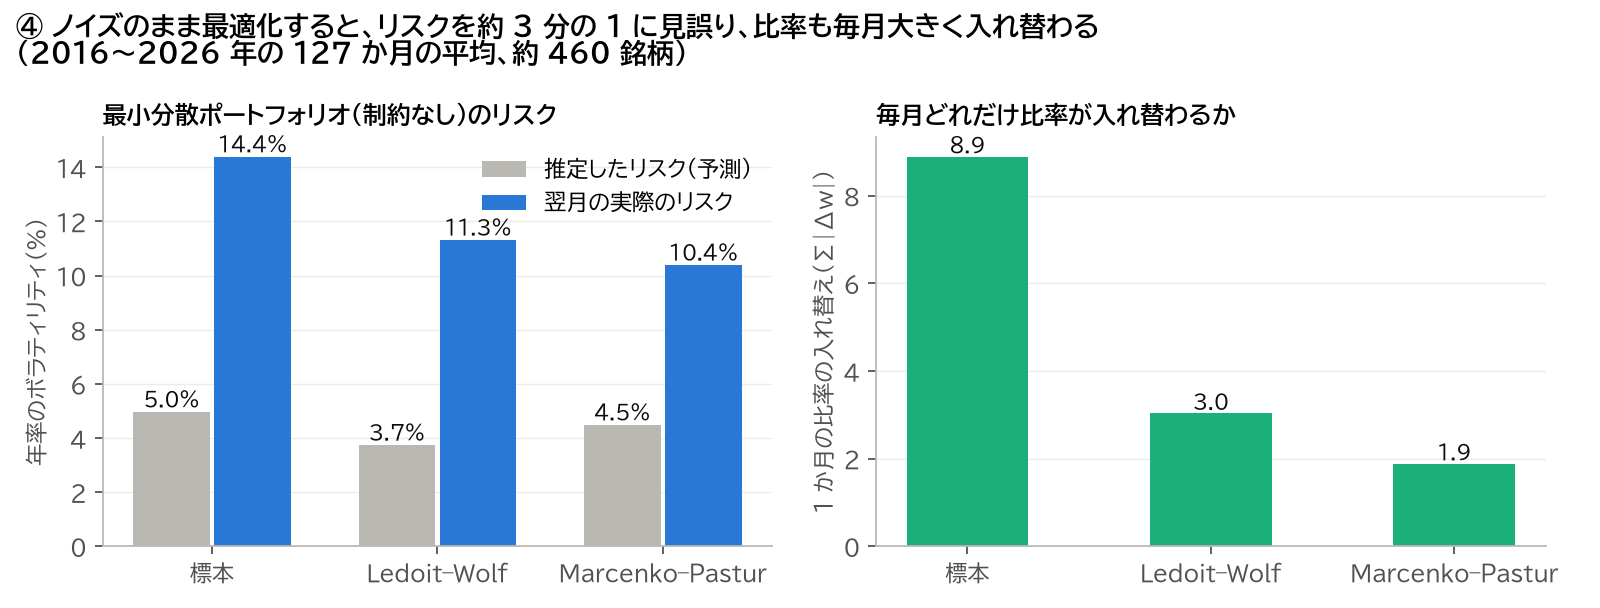
\includegraphics[width=0.98\linewidth]{x01_4_outcome.png}
\caption{制約のない最小分散ポートフォリオ。そのままの標本共分散ではリスクを約 3 分の 1 に見誤り、比率も毎月大きく入れ替わる。}
\end{figure}

\begin{table}[H]
\centering
\caption{翌月の実際のリスク（年率）。}
\small
\begin{tabular}{lrrr}
\toprule
& 標本 & Ledoit--Wolf（今の BLM） & Marcenko--Pastur \\
\midrule
制約のない最小分散：ボラティリティ & 14.4\% & 11.3\% & \textbf{10.4\%} \\
空売りなしの最小分散：ボラティリティ & 10.5\% & \textbf{10.5\%} & 10.6\% \\
BLM の最適化（TE の上限 3\%）：実際の TE & 4.8\% & \textbf{4.5\%} & 4.7\% \\
\bottomrule
\end{tabular}
\end{table}

\begin{itemize}
\item 制約のない最適化では、ノイズ除去がはっきり効く（実際のリスク 11.3\% $\to$ 10.4\%、$t$ $-5.8$）。
\item 空売りの禁止や TE の上限があると、制約そのものがノイズによる大きな賭けを抑えるので、差はほとんど消える。BLM の最適化では Ledoit--Wolf がわずかに良かった（$+0.14$ ポイント、$t$ 3）。\textbf{BLM の共分散は今のままでよい。}
\item どの推定でも、実際の TE は上限 3\% の約 1.5 倍になった。過去 1 年から推定した共分散は、翌月のリスクの変化を捉えきれない。BLM の結果を報告するときは、上限ではなく実際の TE を書く。
\end{itemize}

% ============================================================
\chapter{再現の手順と記録}\label{app:repro}

\begin{table}[H]
\centering
\caption{ブランチ \code{feature/earnings-events} の主なコミット（すべて GitHub にプッシュ済み）。}
\small
\begin{tabular}{ll}
\toprule
コミット & 内容 \\
\midrule
\code{f7d3bba} & 設計（\code{設計.md}：ディレクトリ、表、時刻、点数、評価の順番） \\
\code{792766c} & 実装（表、EDGAR の取得、時刻、数値の驚き、点数、統計）と H06 の移し替え \\
\code{d81b6fc} & ChronoGPT の点数付けの修正（GPU のメモリ） \\
\code{867ddbd}、\code{bc8c6d9} & X01（共分散のノイズ除去）と図 \\
\code{2df746e} & \textbf{事前登録と評価のコード（反応を計算する前）} \\
\code{94e08f8} & E2 の結果 \\
\bottomrule
\end{tabular}
\end{table}

\begin{verbatim}
python run_events.py import-h06        # H06 の結果を DB へ
SEC_USER_AGENT="<名前> <メール>" \
  python run_events.py fetch --from 2015-01-01 --to 2023-10-31
python run_events.py surprise          # 数値の驚き
python run_events.py score dictionary  # finbert / chrono も同じ
python experiments/E2_event_reaction/run.py   # 事前登録の後に 1 回だけ
python 資料集/02_実験/実験2_決算発表文/作成スクリプト/figs.py   # この資料の図
\end{verbatim}

費用は gpt-4o-mini の 3.31 ドル（前回の H06 のもの）だけで、今回の点数付けと評価はすべてこの PC で行った（GPU で約 13 時間）。

% ============================================================
\chapter*{参考文献}
\addcontentsline{toc}{chapter}{参考文献}

\begin{itemize}\small
\item Chen, S., Green, T. C., Gulen, H., Zhou, D. (2024). What Does ChatGPT Make of Historical Stock Returns? arXiv:2409.11540.
\item He, S., Lv, L., Manela, A., Wu, J. (2025). Chronologically Consistent Large Language Models. arXiv:2502.21206.
\item He, S., Lv, L., Manela, A., Wu, J. (2025). Instruction Tuning Chronologically Consistent Language Models. arXiv:2510.11677.
\item Huang, A. H., Wang, H., Yang, Y. (2023). FinBERT: A Large Language Model for Extracting Information from Financial Text. Contemporary Accounting Research 40(2).
\item Jagannathan, R., Ma, T. (2003). Risk Reduction in Large Portfolios: Why Imposing the Wrong Constraints Helps. Journal of Finance 58(4).
\item Kolari, J. W., Pynnönen, S. (2010). Event Study Testing with Cross-Sectional Correlation of Abnormal Returns. Review of Financial Studies 23(11).
\item Lopez-Lira, A., Tang, Y., Zhu, M. (2025). The Memorization Problem: Can We Trust LLMs' Economic Forecasts? arXiv:2504.14765.
\item López de Prado, M. (2020). Machine Learning for Asset Managers. Cambridge University Press.
\item Loughran, T., McDonald, B. (2011). When Is a Liability Not a Liability? Journal of Finance 66(1).
\item Siano, F. (2025). The News in Earnings Announcement Disclosures: Capturing Word Context Using LLM Methods. Management Science 71(11).
\item Wu, Y., Akin, E. M., Martineau, C., Grégoire, V., Veneris, A. (2025). Extracting the Structure of Press Releases for Predicting Earnings Announcement Returns. arXiv:2509.24254.
\item Yu, D., Liu, Z., Zhang, H., He, H. (2026). Fast Numbers, Slow Language: Bridging Quantitative and Qualitative Earnings Signals. arXiv:2606.29734.
\end{itemize}

\end{document}
